\chapter{Routing}
Das Routing umfasst das Suchen des schnellsten Weges zwischen zwei Knoten eines Netzwerkes. Es ist nicht zu verwechseln mit dem Weiterleiten (engl. Forwarding), welches sich genau genommen nur mit dem Weiterleiten von Nachrichten beschäftigt, unter der Annahme, dass bereits der kürzeste Weg bekannt ist. Diese beiden Aufgaben hängen jedoch insofern zusammen, als dass für das Weiterleiten einer Nachricht der kürzeste Weg bekannt sein muss. Daher, und weil Routing-Protokolle meist auch die Weiterleitung übernehmen, werden Routing und Weiterleiten oft als Synonyme verwendet. Die zentrale Aufgabe des Routings ist es, eine Routingtabelle (Weiterleitungstabelle) zu erstellen. Diese Tabelle enthält für jeden bekannten Knoten den kürzesten Weg, genauer gesagt den nächsten Knoten des kürzesten Weges zum Ziel. Diese Weiterleitungstabelle wird, wie der Name vermuten lässt, beim Weiterleiten von Nachrichten verwendet, um den nächsten Knoten (den nächsten Hop) zu bestimmen. Die Metrik, welche für die Bestimmung des kürzesten Weges verwendet wird, wird als Kosten bezeichnet. Jeder Kante im Netzwerkgraph werden bestimmte Kosten zugeordnet. Diese Kosten können sich aus mehreren Eigenschaften wie beispielsweise der Übertragungsleistung, der Zuverlässigkeit oder ähnlichem zusammensetzen. In diesem vereinfachten Beispiel werden als Kosten die Distanz zum nächsten Knoten genommen. Somit hat jede Kante im Netzwerkgraph einen Kostenwert von 1.\footcite{distsys1}

\section{Routing-Algorithmen}
Um die oben genannten Aufgaben zu erfüllen wurden im Laufe der Zeit eine Vielzahl von Algorithmen mit unterschiedlichen Eigenschaften entworfen. Es gibt verschiedene Ansätze die sich in Aufbau, Anpassungsfähigkeit und allgemeiner Funktionsweise unterscheiden. In den folgenden Sektionen wird die Aufteilung der Verfahren und ihre Unterschiede besprochen.

\subsection{Statisches Verfahren}
Dieses Verfahren ist das simpelste, jedoch in der Praxis kaum anwendbar. Die Weiterleitungstabelle eines jeden Knoten wird beim Aufsetzen des Netzwerks einmalig angelegt, danach kann diese nur noch manuell geändert werden. Aufgrund der statischen Eigenschaft dieses Verfahrens können temporäre Ausfälle von Knoten nur schwer berücksichtigt werden, daher wird es nur wenn überhaupt für provisorische Netzwerke mit simpler, sich kaum verändernder Topologie verwendet.

\subsection{Zentrale Verfahren}
Hier liegt die Routingtabelle bei einer zentralen Kontrolleinheit, welche sie an alle Knote weitergibt. Änderungen im Netzwerk müssen von der Zentrale erkannt werden und an alle Knoten weitergegeben werden. Um dies zu ermöglichen muss der Zentrale das gesamte Netzwerk bekannt sein und eine entsprechende Leistung und Ausfallsicherheit gegeben sein. Wie bei allen zentral geregelten Algorithmen ist ein Single-Point-of-Failure gegeben, welcher bei einem Ausfall das gesamte System lahmlegen kann.

\subsection{Isolierte Verfahren}
Im Unterschied zu den meisten Routing-Verfahren werden bei isolierten Verfahren keine Routing-Informationen zwischen den Knoten des Netzwerkes versendet. Jeder Knoten ist so gesehen auf sich allein gestellt und kann nur auf die ihm direkt zu Verfügung stehenden Informationen zugreifen. Ein Beispiel für solch eine Information ist die Größe der Warteschlangen an den Ausgängen des Knoten. Zu den isolierten Verfahren zählt auch das sogenannte Hot-Potato-Verfahren (Heiße Kartoffel). Dabei ist das Ziel des Knoten, ein erhaltenes Paket möglichst schnell wieder weiter zusenden. Dadurch hat zwar jeder Knoten einen geringen Rechenaufwand, jedoch kann es bei Paketen zu sehr großen Verzögerungen kommen.

\subsection{Verteilte Verfahren}
Bei einem verteilten Verfahren gibt es, wie bei anderen verteilten Systemen, keine zentrale Steuereinheit. stattdessen ist jeder Knoten selbst für seinen Teil des Rouings verantwortlich und besitzt damit auch seine eigene Weiterleitungstabelle. Genauer werden diese Verfahren auch als verteilte adaptive Verfahren bezeichnet, da sie sich an Ausfälle im Netzwerk selbstständig anpassen können. Ein zentraler Punkt dieser Verfahren ist der Austausch von Routing-Informationen zwischen den Knoten des Netzwerks. Welche Informationen ausgetauscht werden, hängt vom konkreten Verfahren ab.

\section{Distanzvektor-Algorithmus}
Dieser Algorithmus basiert darauf, dass jeder Knoten eine Tabelle (Vektor) verwaltet, in dem die kürzesten Wege zu den anderen Knoten eingetragen sind. Im Gegensatz zu statischen Verfahren wird diese Tabelle dynamisch vom Knoten selbst erstellt und an Veränderungen im Netzwerk angepasst.

\subsection{Prinzip}
Die Tabelle bzw. der Distanzvektor enthält für jeden dem Knoten bekannten Knoten einen Eintrag (einschließlich des Knoten selbst). Zu jedem dieser Einträge wird der nächste Knoten am Weg und die gesamten Kosten bis zum Ziel gespeichert. Die Kosten sind abhängig von der konkreten Implementierung im Routing-Protokoll, für dieses Beispiel werden die Anzahl der Knoten (der Hop-Count) als Kosten verwendet. Der Graph in Abbildung \ref{fig:network_graph} zeigt ein Beispielnetzwerk, anhand dessen dieser Algorithmus erklärt wird. In diesem Beispiel gehen wir davon aus, dass jeder Knoten nur seine direkten Nachbarn und nicht das gesamte Netzwerk kennt. Er muss daher nicht nur die Kosten für jeden Knoten, sondern auch die Knoten an sich speichern.

\begin{figure}
    \centering
    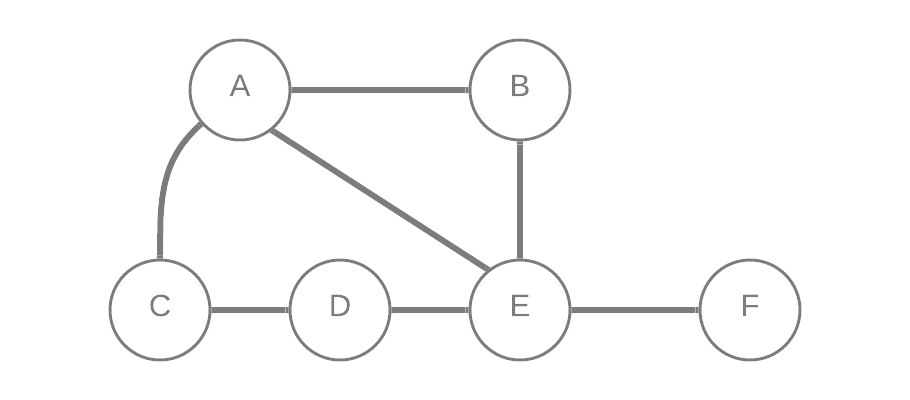
\includegraphics[width=\textwidth]{images/distance_vec_example_1.png}
    \caption{Beispiel eines Netzwerkgraphen}
    \label{fig:network_graph}
\end{figure}

Das Prinzip dieses Algorithmus ist simpel. Zu Beginn werden alle direkten Nachbarn des Knoten und der Knoten selbst in die Tabelle eingetragen. Am Beispiel betrachtet trägt der Knoten A somit B, C und E als seine Nachbarn ein. Zu jedem dieser Nachbarn sind die Kosten gleich 1. Sich selbst trägt der Knoten mit den Kosten von 0 ein. Die Tabelle \ref{example_start} zeigt, wie der Distanzvektor nun in diesem Beispiel aussieht.

\begin{table}
\caption{Beispiel des Distanzvektor am Beginn}
\label{example_start}
\centering
\begin{tabular}{| c | c | c |}
\hline
\textbf{Ziel} & \textbf{Kosten} & \textbf{Nächster Knoten} \\
\hline
A & 0 & A \\
\hline
B & 1 & B \\
\hline
C & 1 & C \\
\hline
E & 1 & E \\
\hline
\end{tabular}
\end{table}

Die im Vektor gespeicherten Informationen werden nun an alle Nachbarn weitergeleitet. Wenn ein Knoten von seinem Nachbarn einen Vektor erhält, wird dieser mit dem gespeicherten verglichen. Ist für einen Knoten noch kein Eintrag vorhanden, werden die erhaltenen Werte übernommen, wobei die Kosten um eins erhöht werden. Gibt es für ein Ziel bereits einen Eintrag, werden die Kosten verglichen. Sind die um eins erhöhten Kosten des erhaltenen Vektors kleiner, wird der Nachbar, von dem der Vektor stammt, als nächster Knoten eingetragen  und die Distanz angepasst. Wenn in unserem Beispiel nun A den Vektor von C erhält sieht der neue Vektor von A wie in Tabelle \ref{example_step_1} dargestellt aus. Dieser Vorgang geschieht bei jedem Knoten, bis schließlich alle Routen bekannt und im Distanzvektor eingetragen sind. Der endgültige Vektor kann für dieses Beispiel etwa so aussehen wie in Tabelle \ref{example_final}

\begin{table}
\caption{Beispiel des Distanzvektors nach erstem Update}
\label{example_step_1}
\centering
\begin{tabular}{| c | c | c |}
\hline
\textbf{Ziel} & \textbf{Kosten} & \textbf{Nächster Knoten} \\
\hline
A & 0 & A \\
\hline
B & 1 & B \\
\hline
C & 1 & C \\
\hline
E & 1 & E \\
\hline
D & 2 & C \\
\hline
\end{tabular}
\end{table}

\begin{table}
\caption{Beispiel des Distanzvektors am Ende}
\label{example_final}
\centering
\begin{tabular}{| c | c | c |}
\hline
\textbf{Ziel} & \textbf{Kosten} & \textbf{Nächster Knoten} \\
\hline
A & 0 & A \\
\hline
B & 1 & B \\
\hline
C & 1 & C \\
\hline
E & 1 & E \\
\hline
D & 2 & C \\
\hline
F & 2 & E \\
\hline
\end{tabular}
\end{table}

\subsection{Ausfall einer Verbindung}
Um den Ausfall einer Verbindung anhand unseres Beispiels zu erläutern, nehmen wir an, dass die Verbindung zwischen C und D ausgefallen ist. Wird der Ausfall vom Knoten C erkannt, setzt dieser seine Kosten für den Weg nach D auf Unendlich. Dies teilt er A mit, worauf hin auch A seine Kosten für D aktualisiert und dies E mitteilt. E wird seine Kosten für D jedoch nicht ändern, da E den Knoten D noch direkt erreichen kann. Danach teilt es A mit, dass D über ihn erreicht werden kann. A ändert seinen Eintrag für den nächsten Knoten nach D auf E und kann den Knoten D wieder erreichen.

\subsection{Count-to-Infinity Problem}
Bei dieser Art der Ausfallerkennung kann es jedoch zu einem Problem kommen, dass als Count-to-Infinity (Bis zur Unendlichkeit zählen) bezeichnet wird. Angenommen wird, dass die Verbindung zwischen E und F ausfällt. E setzt somit seine Kosten für F auf den Wert für Unendlich. Wenn nun eine Aktualisierung von B kommt, welche für F die Kosten 2 beinhaltet, wird E diese übernehmen, um eins erhöhen und B als nächsten Knoten eintragen. Diese Information sendet er nun zurück an B, welcher ebenfalls seine Kosten für F um eins erhöht und diese Aktualisierung erneut aussendet. Dieser Vorgang wiederholt sich, bis eine gewisse Schranke erreicht wird, ab der abgebrochen wird. Je nach Höhe dieser Schranke und Häufigkeit der Aktualisierungen kann es zu beträchtlichen Verzögerungen kommen, bis ein Ausfall erkannt wird. Um dieses Problem zu umgehen gibt es die Verbesserung des Split Horizon (geteilter Horizont). Diese Verbesserung legt fest, dass ein Knoten keine Aktualisierungen an den Knoten zurückschickt, von dem er den Wert erhalten hat. Dadurch werden jedoch nur Schleifen mit zwei Knoten vermieden.\footcite{distsys1}